\documentclass[12pt]{report}
\usepackage{setspace}
\usepackage{amsmath,amssymb}
\usepackage{amsfonts}
\usepackage{graphicx}
\usepackage[pdftex,bookmarks=true,bookmarksopen=false,bookmarksnumbered=true,colorlinks=true,linkcolor=black]{hyperref}
\usepackage{float}
\usepackage[utf8]{inputenc}

\begin{document}

\begin{titlepage}
\begin{center}
{\LARGE Getulio Vargas Foundation}\\
\vspace{0.3cm}
{\LARGE Applied Mathematics School}\\
\vspace{0.3cm}

\par
\vspace{170pt}
  \textbf{\Large {Machine learning aproach for Dengue forecasting - Comparing LSTM, Random Forest and Lasso}}\\
  
\vspace{32pt}
{\Large Elisa Mussumeci}\\
\end{center}

\par
\vfill
\begin{center}
{{\normalsize Rio de Janeiro}\\
{\normalsize \the\year}}
\end{center}
\end{titlepage}

\thispagestyle{empty}

\newpage
\begin{center}
\textbf{\LARGE Elisa Mussumeci}

\par
\vspace{200pt}
\textbf{\Large Machine learning aproach for Dengue forecasting - Comparing LSTM, Random Forest and Lasso}
\end{center}

\par
\vspace{85pt}
\hspace*{175pt}\parbox{7.6cm}{{\normalsize Dissertação submetida à Escola de Matemática Aplicada como requisito parcial para a obtenção do grau de Mestre em Modelagem Matemática da Informação.}}

\par
\vspace{1em}
\hspace*{125pt}\parbox{10.0cm}{{\normalsize Área de Concentração: }}

\par
\vspace{1em}
\hspace*{125pt}\parbox{10.0cm}{{\normalsize Orientador: Flávio Codeço Coelho}}\\

\par
\vfill
\begin{center}
{{\normalsize Rio de Janeiro}\\
{\normalsize \the\year}}
\end{center}

\thispagestyle{empty}

\newpage
\noindent{\textbf{\large Acknowledgements}}\\
\doublespacing
Gostaria de agradecer....

\thispagestyle{empty}

\newpage
\begin{center}
\textbf{\normalsize Resumo}
\end{center}
\vspace{1pt}

resumo...

\thispagestyle{empty}

\newpage
\begin{center}
\textbf{\normalsize Abstract}
\end{center}
\vspace{1pt}

We use the Infodengue database of incidence and climate time-series, to train predictive models for the weekly number of cases of dengue in 733 cities of Brazil. To overcome limitation in the length of timeseries available to train the model, we included the time series of similar cities as predictors in the model of each city. The LSTM recurrent neural network model attained the highest performance in predicting future incidence on dengue in cities of different sizes. 

\thispagestyle{empty}

\newpage
\tableofcontents
\listoffigures
\thispagestyle{empty}

\newpage
\chapter{Introduction}

Understanding and therefore being able to predict the incidence of seasonal diseases is a big challenge due in part to the complex cycles these diseases display but also to  incomplete records of historical disease incidence and other cofactors affecting risk. Besides the cycles are strongly influenced by local climate  and other contextual variables making it hard to extrapolate findings from one geographical area to another.

For vector-borne diseases, the complexity is compounded by the coupling of the transmission of the dynamics in humans with the population dynamics of the vector species.

Having complete datasets for large geographical areas can help this effort as one can study the effects of spatial and climatic gradients on the intrinsic dynamics of disease transmission. 

In this paper, we use the Infodengue[ref] database of more than 700 municipalities of Brasil to develop predictive models capable of predicting the weekly incidence of Dengue in various regions of Brazil across a wide range of latitudes and climate characteristics.

\newpage
\chapter{Literature Review}

\section{Epidemic forecasting}
 
Time series forecasting consists in use models to predict future values based on previously observed values.
 
 
In epidemiology studies, forecasting is important to understand disease spread over a period of time

It's commom to use time series forecasting models to predict epidemic
 
The most comon models used for epidemic forecasting are:
 
 \begin{description}
  \item Autoregressive Integrated Moving Average (ARIMA)
  \item Seasonal Autoregressive Integrated Moving Average (SARIMA)
  \item VAR
 \end{description}

 
\subsection{Multi time series forecast}

Apresentar a diferença entre predição de series temporas simples e multiplas. Explicar cada modelo que vem sendo utilizado em prediçao multipla

\subsection{Data modeling and cluster analysis}


\section{Machine Learning and forecasting}

machine learning is bla bla

machine learning techniques have been used to forecast as show in ref and ref. It bring good results since
it cand bla bla ref.

Neural networks is one technique that has been researched quite 
extensively, and has often been shown to beat time series approaches ref 

explain why these kind of models are good for forecasting

\subsection{Random Forest and Lasso}

\begin{description}
 \item Random Forest
  
 Random forests  are an ensemble learning method for classification, 
 regression and other tasks, that operate by constructing a multitude of decision trees at training time 
 and outputting the class that is the mode of the classes (classification) or mean prediction (regression) 
 of the individual trees.
 
 Decision tree learning is a method commonly used in data mining. The goal is to create a model 
 that predicts the value of a target variable based on several input variables. 
 
 The difference between Random Forest algorithm and the decision tree algorithm is that in 
 Random Forest, the process es of finding the root node and splitting the feature nodes will run
 randomly.
 
 Add formula
 
 \item Lasso
 
 In statistics and machine learning, lasso (least absolute shrinkage and selection operator)
 (also Lasso or LASSO) is a regression analysis method that performs both variable selection and
 regularization in order to enhance the prediction accuracy and interpretability of the statistical
 model it produces. It was introduced by Robert Tibshirani in 1996 based on Leo Breiman’s
 nonnegative garrote.
 
 Lasso was originally introduced in the context of least squares, and it can be instructive to consider 
 this case first, since it illustrates many of lasso’s properties in a straightforward setting.
 
\end{description}


\subsection{Long-short term memory (LSTM)}

Recurrent neural networks ADD REF are neural networks with loops in them, allowing information
to persist. They can be thought of as multiple copies of the same network, each passing a message
to a successor.

RNN's have great performance  in most cases but they can't handle long-term dependencies. That 
means that when the gap between the relevant information and the output is too large, the network
become unable to learn to connect the information.

Long Short Term Memory networks (add ref )are a special kind of RNN, capable of learning
such long-term dependencies. In each cell of chain the network decides whoch informations to keep
and which to forget, etcs

add colah diagram step by step

\newpage
\chapter{Article}

\section{Methodology}


\subsection{Data sources}

The data used in the article was collected from the infodengue project. 

The infodengue project \cite{codeco2016infodengue} is a alert system of the number of dengue cases registered in the 
cities of Brazil, aiming to provide  information to the population.

This dataset consist information are provided by the health secreaty of each city, and consists of 
incidence, minimum and maximum temperature, minimum and maximum humidity and 
atmospheric pressure series for each week. The data if from 2011 until nowday (fix).

Add states and number of cities of each one 

Add example of data.

\subsection{Data modeling}

Some cities have the incidence series very similar, what makes us thing that using the information 
of cities nearby or with similar climate may have some influence in the number of dengue cases.

ADD SOME GRAPH 

In order to input the maximum number o relevant information to the model without overload the model,
we clustered the data based on the correlation distances between incidence time series within each state.

add the formula of the correlation used, add

talk about hierarquical clustering and the treshold used, image example of a h cluster.

For each city, a feature matrix was assembled from the set of time series of 
each other time series from its cluster.

matrix example of the data clustered

A single city model was trained for a few selected cities to serve as a 
baseline against which to compare the effectiveness of the using sister 
cities (within the same cluster) cluster as predictors.

\subsection{Forecasting}

We tried tree diferent models bla bla


\begin{description}
 \item \textbf{Random Forest}
 
 falar sobre modelagem, 
 \item \textbf{Long short term memory (LSTM)}
 
 A LSTM model was defined with topology given in table xx. the model was trained 
for 300 epoch using a custom loss function defined in equation (xx) A look back 
of 4 weeks a forecasting window of 10 weeks were chosen.

 
 \item \textbf{Lasso}
 
\end{description}


\section{Results}

\subsection{Cluster analysis}
The cluster found within each state are shown in figures ... The clusters can 
also be seen in the map in figures xxx.
\begin{figure}[h]
 \centering
 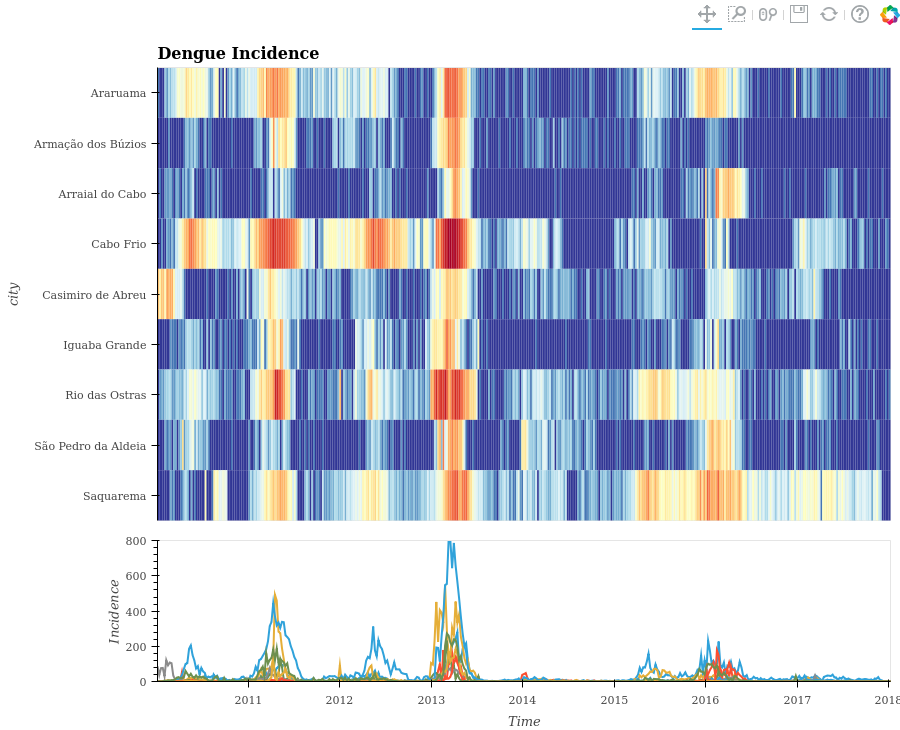
\includegraphics[scale=0.4]{./cluster_3300209.png}
 % cluster_3300209.png: 0x0 pixel, 300dpi, 0.00x0.00 cm, bb=
 \caption{cluster}
\end{figure}

\subsection{Forecasting}

Figures xx and yy show the performance of the prediction  both \emph{in-sample} 
and  \emph{out-of-sample}.

forecasting with cluster and without cluster?

\section{Discussion}

The model has show good performance for both large and small cities from 
various parts of Brasil. This shows that the set of predictor series selected 
is capable to characterize the epidemic dynamics.

The extra information provided by the sister cities' series alowed the 
model to substantially outperform the base model. The LSTM model was 
capable of consistently predict the incidence pattern of non-epidemic years. 

\newpage
\chapter{Conclusions and Final Considerations}

\newpage
\phantomsection
\addcontentsline{toc}{chapter}{References}
\bibliographystyle{model1-num-names}
\bibliography{sample}

\newpage
\phantomsection
\addcontentsline{toc}{chapter}{Appendices}
llalalala

\end{document}